\documentclass{book}
\usepackage[margin=1in]{geometry}
% Standard Packages
\usepackage{amsmath, amssymb, graphicx} 
\usepackage{epigraph, xcolor, framed, cite} % For formatting, references
\usepackage{microtype} % Improves typography
\usepackage{hyperref} % Creates clickable links/references

\usepackage{tikz}
\usetikzlibrary{shapes, arrows.meta, positioning, circuits.ee.IEC}
\tikzstyle{every node}=[font=\small] % Optional: smaller font size for labels

% Hyperref Setup (optional colors)
\hypersetup{
    colorlinks=true,
    linkcolor=blue,
    filecolor=magenta,      
    urlcolor=cyan,
    citecolor=green
}

% Epigraph settings (from original)
\renewcommand{\textflush}{flushright}
\renewcommand{\sourceflush}{flushright}
\renewcommand{\epigraphsize}{\large}
\setlength{\epigraphwidth}{.7\textwidth}

% Define framed environment for Key Results (from original)
\definecolor{examplebgcolor}{rgb}{0.95, 0.95, 0.95} % Background color not used here, but defined
\newenvironment{keyresult}[1][Key Result]{\begin{framed}\noindent\textbf{#1:}}{\end{framed}}

% Define a simple problem environment for clarity
\newenvironment{problem}[1][Problem]{\par\medskip\noindent\textbf{#1:}\em}{\par\medskip}

% Chapter setup - start numbering appropriately
\setcounter{chapter}{5} 
\renewcommand{\thesection}{\thechapter.\arabic{section}} % Standard section numbering: Chapter.Section

% --- Document Starts ---
\begin{document}

% --- NEW INTRODUCTORY SECTION ---
\chapter*{Setting the Stage: A Quantum Tug-of-War}
\label{chap:prologue}

\epigraph{\textit{The transition is everything.}}{Lynda Barry}

This chapter is about a fascinating little quantum system – a superconducting circuit known as the Cooper Pair Box. Why study it? Well, apart from being a beautiful example of quantum mechanics in action, variations of this circuit are workhorses in modern quantum computing efforts, forming the basis for qubits. Our journey will take us through the physics governing this system, revealing how its behavior dramatically shifts depending on which physical effect dominates.

At its heart, this is a story of competition, a quantum tug-of-war between two fundamental energies:
\begin{enumerate}
    \item \textbf{Charging Energy ($E_C$):} Think of this like an energy cost for having charge on a small island. Nature often prefers neutrality, and $E_C$ quantifies the penalty for deviating from that. This term favors states where the number of charges (here, Cooper pairs, charge \(2e\)) is precisely known.
    \item \textbf{Josephson Energy ($E_J$):} This energy arises from the quantum mechanical tunneling of Cooper pairs across a weak link (the Josephson junction). It depends on the *phase* difference \(\phi\) across that junction, creating a potential landscape that prefers certain phase values.
\end{enumerate}

The entire personality of the Cooper Pair Box hinges on the ratio \(E_J / E_C\). When charging energy wins (\(E_C \gg E_J\)), the system behaves like a "charge qubit," exquisitely sensitive to charge. When Josephson energy wins (\(E_J \gg E_C\)), it morphs into a "transmon qubit," much more robust against charge fluctuations, but still quantum mechanical enough to be useful.

Our main tool is the Hamiltonian, the operator that dictates the system's energy and evolution:
\[ \hat{H} = 4 E_C (\hat{N} - n_g)^2 - E_J^{(1)} \cos \hat{\phi} - \frac{E_J^{(2)}}{2} \cos (2 \hat{\phi}) \]
Here, \(\hat{N}\) is the operator for the number of Cooper pairs (our "charge"), and \(\hat{\phi}\) is the operator for the phase difference. They are conjugate variables, like position and momentum, obeying \([\hat{\phi}, \hat{N}] = i\) (we'll mostly use units where \(\hbar = 1\)). The parameter \(n_g\) is an experimentally controlled "gate charge" that allows us to tune the system's preference, and \(E_J^{(1)}, E_J^{(2)}\) represent potentially different Josephson energy scales (often, \(E_J^{(2)}\) is small or zero, but we'll keep it for generality).

Our plan is to dissect this Hamiltonian. We'll start by analyzing the two extreme limits – large \(E_C\) and large \(E_J\) – using familiar quantum mechanical tools like perturbation theory and the harmonic oscillator approximation. Then, we'll examine a special case where an exact solution reveals the smooth transition between these regimes. Finally, we'll step back and interpret what it all means in the context of building better qubits. Let's begin!



% --- MAIN CHAPTER CONTENT ---
\chapter{The Cooper Pair Box: From Charge Qubit to Transmon}
\label{chap:cpb}

% Note: The original chapter epigraph is now in the prologue. 
% You could add a new one here if desired.

\noindent\textit{Note on units:} We continue to use units where \(\hbar = 1\), except where restoring it aids clarity.


\section{The Quantum Variables: Phase and Charge}
\label{sec:intro} % Renamed for clarity

Let's formalize our quantum players. The core degree of freedom is the superconducting phase difference \(\hat{\phi}\), which behaves mathematically like an angle, confined to \(\phi \in [-\pi, \pi)\). Its conjugate partner is the charge operator \(\hat{N}\), which counts the number of excess Cooper pairs (fundamental charge \(2e\)) residing on a small superconducting "island" (see Figure~\ref{fig:cpb_schematic}). Because \(\phi\) is an angle, adding \(2\pi\) shouldn't change the physics, a periodicity inherent in the system.

\begin{figure}[h]
    \centering
    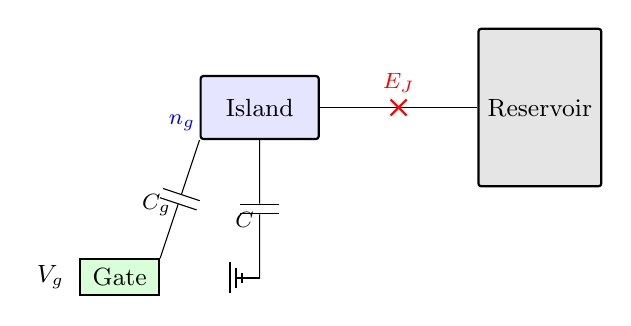
\begin{tikzpicture}[
        circuit ee IEC,
        node distance=1cm and 1.5cm, % Adjusted default distances
        font=\small, % Apply small font globally
        island/.style={draw, thick, minimum width=1.5cm, minimum height=0.8cm, fill=blue!10, rounded corners=1pt},
        reservoir/.style={draw, thick, minimum width=1cm, minimum height=2cm, fill=gray!20, rounded corners=1pt},
        gate/.style={draw, thick, minimum width=1cm, minimum height=0.3cm, fill=green!15}
    ]

    % --- Nodes ---
    \node[island] (island) {Island};
    \node[reservoir, right=2cm of island] (res) {Reservoir};
    \coordinate (ground_coord) at ([yshift=-1.75cm]island.south);
    \node[gate, below left=1.5cm and 0.5cm of island] (gate) {Gate};

    % --- Connections & Labels ---

    % 1. Josephson Junction (Island <-> Reservoir)
    \coordinate (jj_pos) at ($(island.east)!0.5!(res.west)$);
    \draw (island.east) -- (jj_pos);
    \draw (jj_pos) -- (res.west);
    \node at (jj_pos) [draw, cross out, minimum size=5pt, thick, red, inner sep=0pt] {};
    \node at (jj_pos) [above=2pt, font=\footnotesize, red] {$E_J$};

    % 2. Island Capacitance to Ground
    % Draw the capacitor path first, naming it 'capC'
    \draw (island.south) to[capacitor={name=capC}] (island.south |- ground_coord);
    % Place the label 'C' as a separate node relative to the capacitor path
    \node[below left, font=\footnotesize, inner sep=1pt, xshift=-1pt] at (capC.center) {$C$}; % Position relative to center, shifted slightly
    \draw[thick] (island.south |- ground_coord) -- ++(-0.3cm,0) node[ground, scale=0.8]{};

    % 3. Gate Capacitance (Gate <-> Island)
    % Draw the capacitor path first, naming it 'capCg'
    \draw (gate.north east) to [capacitor={name=capCg}] (island.south west);
    % Place the label 'Cg' as a separate node relative to the capacitor path
    \node[below left, font=\footnotesize, inner sep=1pt, yshift=3pt, xshift=-2pt] at (capCg.center) {$C_g$}; % Position relative to center, shifted slightly

    % 4. Gate Voltage Label
    \node[left=2pt of gate] {$V_g$};

    % 5. ng Label
    \node[above left=0pt and -2pt of island.south west, font=\footnotesize, text=blue] {$n_g$};


    \end{tikzpicture}
    \caption[Corrected Schematic of a Cooper Pair Box]{A corrected schematic representation of a Cooper Pair Box. The superconducting island connects to a reservoir via a Josephson junction ($E_J$). It has capacitance $C$ to ground and $C_g$ to the gate electrode. The gate voltage $V_g$ tunes the offset charge $n_g$ via $C_g$. The charging energy $E_C = (2e)^2 / (2 C_\Sigma)$ depends on the total capacitance $C_\Sigma = C + C_g + C_J$.}
    \label{fig:cpb_schematic}
\end{figure}

The fundamental quantum mechanical relationship between phase and charge is their commutation relation:
\begin{equation}
[\hat{\phi}, \hat{N}] = i 
\label{eq:commutator}
\end{equation}
This is identical in form to \([\hat{x}, \hat{p}] = i\), and carries the same profound implication: the Heisenberg Uncertainty Principle. You cannot simultaneously know both the phase and the charge number with perfect accuracy. If you know \(N\) precisely, \(\phi\) is completely uncertain, and vice-versa. In the common "phase representation," where wavefunctions depend on \(\phi\), the operators act as you might expect: \(\hat{\phi}\) just multiplies by \(\phi\), while \(\hat{N}\) becomes the derivative operator \(\hat{N} = -i \frac{d}{d\phi}\).

The system's energy is captured by the Hamiltonian we saw earlier:
\begin{equation}
\hat{H} = 4 E_C (\hat{N} - n_g)^2 - E_J^{(1)} \cos \hat{\phi} - \frac{E_J^{(2)}}{2} \cos (2 \hat{\phi})
\label{eq:hamiltonian}
\end{equation}

Let's reiterate the parameters:
\begin{itemize}
    \item \(E_C = (2e)^2 / (2C)\): The charging energy scale, determined by the island's total capacitance \(C\). The \(4 E_C \hat{N}^2\) part acts like kinetic energy (\(\sim p^2/2m\)) in the particle-on-a-ring analogy.
    \item \(n_g\): The dimensionless gate charge, controlled by an external voltage \(V_g\). It acts like a background offset, influencing which charge state \(N\) is energetically cheapest.
    \item \(E_J^{(1)}, E_J^{(2)}\): Josephson coupling energies. They determine the strength of Cooper pair tunneling and create the potential energy landscape \(V(\phi) = -E_J^{(1)} \cos \phi - \frac{E_J^{(2)}}{2} \cos (2 \phi)\) for the phase variable. The \(E_J^{(2)}\) term might arise from circuit complexities or higher harmonics.
    \item \(n_g = \dfrac{C_g V_g}{2e}\): the dimensionless \emph{gate charge}.  
    It tunes the electrostatic offset and therefore which charge state is
    energetically favoured.

\end{itemize}
\medskip
\noindent\textbf{Notation.}  
When the second harmonic is absent we write $E_J\equiv E_J^{(1)}$ and drop
the superscript; $E_J^{(2)}$ is kept explicit only when non-zero.  This
convention avoids clutter while preserving generality.

Our main task is exploring the solutions to the Schr\"odinger equation \[\hat{H}|\psi\rangle = E|\psi\rangle\] in different limits set by the ratio \(E_J / E_C\).

\section{The Stage: Hilbert Space and Operators}
\label{sec:hilbert_space}

Since \(\hat{N}\) corresponds to a physical count of Cooper pairs, its eigenvalues must be integers, \(N \in \mathbb{Z}\). The eigenstates of \(\hat{N}\), denoted \(|N\rangle\), form a natural basis for our Hilbert space. In the phase representation, these are plane waves on the ring:
\begin{equation}
\langle \phi | N \rangle = \psi_N(\phi) = \frac{1}{\sqrt{2\pi}} e^{i N \phi}
\label{eq:charge_eigenstates}
\end{equation}
These states are orthonormal, \(\langle N | M \rangle = \int_{-\pi}^{\pi} \psi_N^*(\phi) \psi_M(\phi) d\phi = \delta_{NM}\), and complete. Any arbitrary state \(|\psi\rangle\) can be written as a superposition \(|\psi\rangle = \sum_N c_N |N\rangle\), corresponding to a \(2\pi\)-periodic wavefunction \(\psi(\phi) = \sum_N c_N (2\pi)^{-1/2} e^{i N \phi}\).

How do our operators act on this basis?
\begin{itemize}
    \item \(\hat{N}\) is simple: \(\hat{N} |N\rangle = N |N\rangle\).
    \item \(\hat{\phi}\) is tricky in the charge basis. It's easier in the phase basis where it's just multiplication by \(\phi\).
    \item \(\cos(k \hat{\phi})\) is interesting. Using Euler's formula, \(\cos(k \phi) = (e^{i k \phi} + e^{-i k \phi})/2\). Since \(e^{i k \phi}\) acting on \(\psi_N(\phi)\) just shifts the index \(N\) to \(N+k\), we find that \(\cos(k\hat{\phi})\) acts as a charge "ladder" operator:\footnote{%
    $e^{ik\hat{\phi}}$ satisfies $e^{ik\hat{\phi}}|N\rangle = |N+k\rangle$, i.e.\ it
    acts as the translation operator in charge space; see
    Koch \textit{et al.}, Phys.\ Rev.\ A \textbf{76}, 042319 (2007).}
    
    \begin{equation}
    \cos(k \hat{\phi}) |N\rangle = \frac{1}{2} \left( e^{ik\hat{\phi}}|N\rangle + e^{-ik\hat{\phi}}|N\rangle \right) = \frac{1}{2} (|N + k\rangle + |N - k\rangle)
    \label{eq:cos_action}
    \end{equation}
    This neatly shows how the Josephson term (\(V(\phi)\)) causes transitions between charge states – it allows Cooper pairs to tunnel on and off the island, changing \(N\).
\end{itemize}
With the mathematical machinery set up, let's explore the first physical limit.

\section[Case 1: Charging Energy Dominates]{Case 1: Charging Energy Dominates (\(E_C \gg E_J\))}
\label{sec:charge_regime}

Imagine \(E_C\) is huge compared to \(E_J^{(1)}\) and \(E_J^{(2)}\). The system cares mostly about minimizing the charging energy term.

\subsection{Ignoring Josephson Tunneling Altogether}
\label{subsec:pure_charging}

If we set \(E_J^{(1)} = E_J^{(2)} = 0\) (no tunneling), the Hamiltonian simplifies dramatically:
\begin{equation}
\hat{H}_0 = 4 E_C (\hat{N} - n_g)^2
\end{equation}
This operator only involves \(\hat{N}\). Its eigenstates are therefore the charge states \(|N\rangle\) themselves, and the energies are simply:
\begin{equation}
E_N^{(0)}(n_g) = 4 E_C (N - n_g)^2
\label{eq:E_N_0}
\end{equation}
These are plotted against the gate charge \(n_g\) in Figure~\ref{fig:charging_levels}. Each energy level forms a parabola, centered at \(n_g = N\). Notice that the parabolas for adjacent charge states (like \(N=0\) and \(N=1\)) cross exactly when \(n_g\) is a half-integer (\(n_g = 1/2, 3/2, \dots\)). At these special "degeneracy points," the system doesn't care energetically whether it has charge \(N\) or \(N+1\).

\begin{figure}[h]
    \centering
    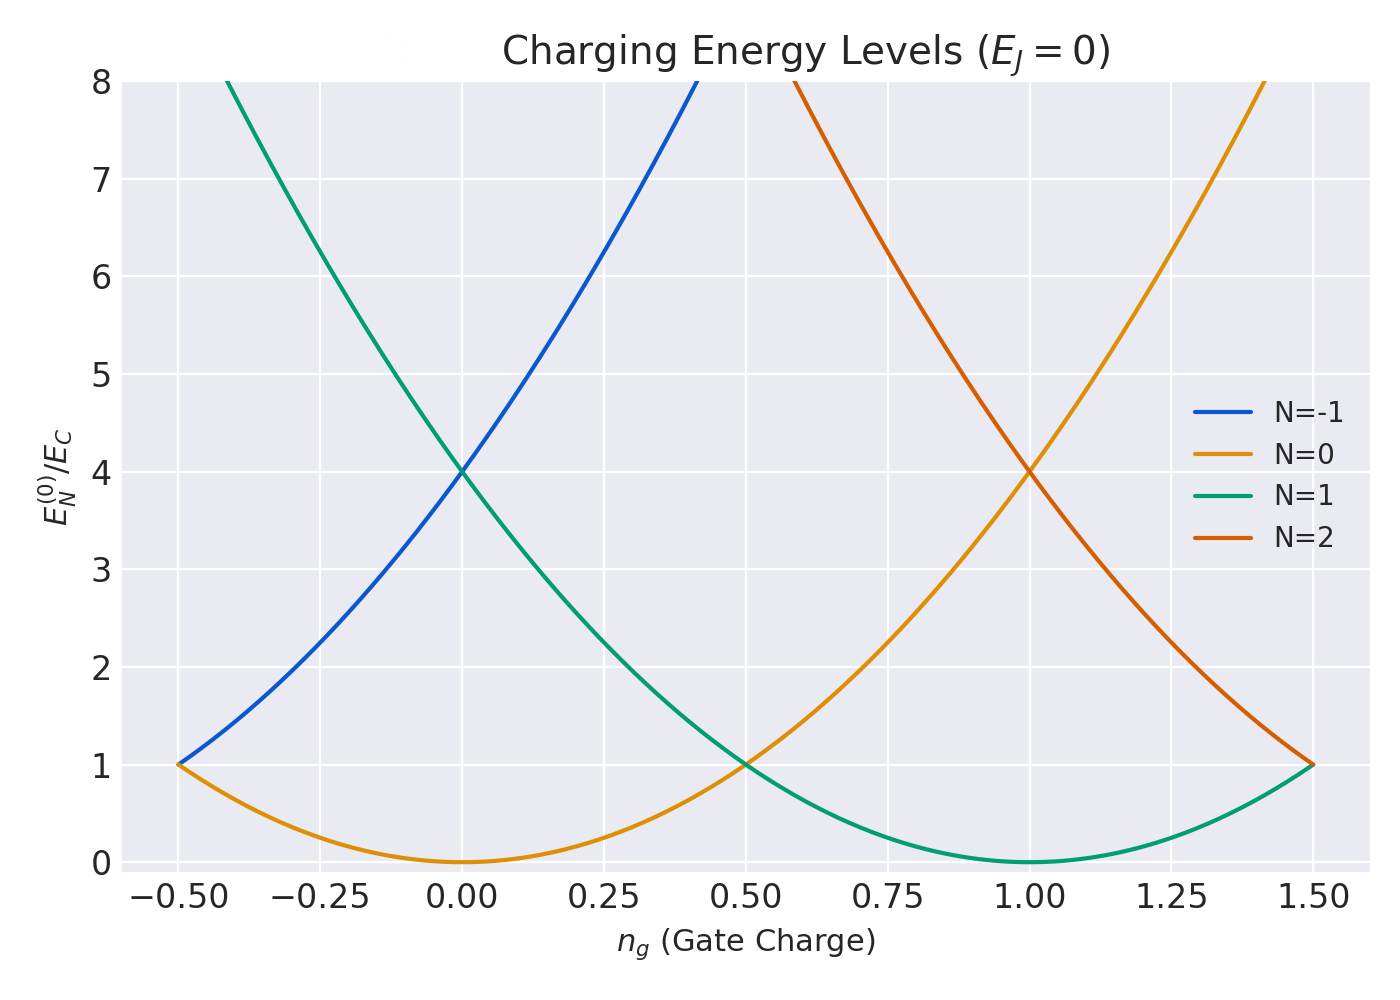
\includegraphics[width=0.8\textwidth]{fig_charge_levels.png}
    \caption[Charging energy levels vs. gate charge]{The energy levels \(E_N^{(0)}\) versus gate charge \(n_g\). Each parabola corresponds to a definite number \(N\) of excess Cooper pairs. Degeneracy occurs where parabolas intersect (e.g., \(N=0\) and \(N=1\) are degenerate at \(n_g=1/2\)).}
    \label{fig:charging_levels}
\end{figure}

\begin{problem}[Problem \ref{chap:cpb}.a.i, Part 1] 
Find the energy eigenvalues and eigenstates of \(\hat{H}_0\). Plot the energy levels versus \(n_g\).
\end{problem}

What about the phase? Since the eigenstate is \(|N\rangle\), its wavefunction is \(\psi_N(\phi) = (2\pi)^{-1/2} e^{i N \phi}\). The probability of finding the phase at a particular value \(\phi\) is:
\begin{equation}
p_N(\phi) = |\psi_N(\phi)|^2 = \left|\frac{1}{\sqrt{2\pi}} e^{i N \phi}\right|^2 = \frac{1}{2\pi}
\end{equation}
It's completely uniform! If you know the charge \(N\) exactly, the phase \(\phi\) is totally undetermined – a perfect illustration of the uncertainty principle at work.

\begin{problem}[Problem \ref{chap:cpb}.a.i, Part 2] 
Determine the probability density \(p(\phi)\) for an eigenstate \(|N\rangle\) and interpret the result.
\end{problem}

\subsection{Turning on Tunneling (as a Perturbation)}
\label{subsec:charging_pert}

Now, let's reintroduce the Josephson terms \(V = -E_J^{(1)} \cos \hat{\phi} - \frac{E_J^{(2)}}{2} \cos (2 \hat{\phi})\), but treat them as a small perturbation, since we assumed \(E_C \gg E_J\). We can use standard perturbation theory. Let's look at the ground state energy at \(n_g = 0\). The unperturbed ground state is \(|0\rangle\), with energy \(E_0^{(0)} = 0\).

The first-order correction to the energy is the expectation value of the perturbation in the unperturbed state:
\begin{equation}
E_0^{(1)} = \langle 0 | V | 0 \rangle = \int_{-\pi}^{\pi} \psi_0^*(\phi) V(\phi) \psi_0(\phi) d\phi = \frac{1}{2\pi} \int_{-\pi}^\pi V(\phi) d\phi
\end{equation}
Since \(\int_{-\pi}^{\pi} \cos(k\phi) d\phi = 0\) for integer \(k \neq 0\), the first-order correction vanishes: \(E_0^{(1)} = 0\). This isn't too surprising; the perturbation averages out over the uniform phase distribution of the \(|0\rangle\) state.

\begin{problem}[Problem \ref{chap:cpb}.a.ii, Part 1] 
Calculate the leading non-zero correction to the ground state energy at \(n_g = 0\).
\end{problem}

To find the leading correction, we must go to second order:
\begin{equation}
E_0^{(2)} = \sum_{N \neq 0} \frac{|\langle N | V | 0 \rangle|^2}{E_0^{(0)} - E_N^{(0)}} = \sum_{N \neq 0} \frac{|\langle N | V | 0 \rangle|^2}{-4 E_C N^2}
\end{equation}
We need the matrix elements \(\langle N | V | 0 \rangle\). Using Eq.~\ref{eq:cos_action}:
\begin{itemize}
    \item \(\langle \pm 1 | V | 0 \rangle = \langle \pm 1 | -E_J^{(1)} \cos\hat{\phi} | 0 \rangle = -E_J^{(1)} \langle \pm 1 | \frac{1}{2}(|1\rangle + |-1\rangle) | 0 \rangle = -E_J^{(1)}/2\)
    \item \(\langle \pm 2 | V | 0 \rangle = \langle \pm 2 | -\frac{E_J^{(2)}}{2} \cos(2\hat{\phi}) | 0 \rangle = -\frac{E_J^{(2)}}{2} \langle \pm 2 | \frac{1}{2}(|2\rangle + |-2\rangle) | 0 \rangle = -E_J^{(2)}/4\)
    \item All other \(\langle N | V | 0 \rangle\) are zero for \(N \neq 0, \pm 1, \pm 2\).
\end{itemize}
Plugging these into the sum (remembering terms for both \(+N\) and \(-N\)):
\begin{equation}
\begin{aligned}
E_0^{(2)} &= \frac{|\langle 1 | V | 0 \rangle|^2}{E_0^{(0)} - E_1^{(0)}} + \frac{|\langle -1 | V | 0 \rangle|^2}{E_0^{(0)} - E_{-1}^{(0)}} + \frac{|\langle 2 | V | 0 \rangle|^2}{E_0^{(0)} - E_2^{(0)}} + \frac{|\langle -2 | V | 0 \rangle|^2}{E_0^{(0)} - E_{-2}^{(0)}} \\
&= \frac{|-E_J^{(1)}/2|^2}{-4E_C (1)^2} + \frac{|-E_J^{(1)}/2|^2}{-4E_C (-1)^2} + \frac{|-E_J^{(2)}/4|^2}{-4E_C (2)^2} + \frac{|-E_J^{(2)}/4|^2}{-4E_C (-2)^2} \\
&= 2 \frac{(E_J^{(1)})^2 / 4}{-4 E_C} + 2 \frac{(E_J^{(2)})^2 / 16}{-16 E_C} \\
&= -\frac{(E_J^{(1)})^2}{8 E_C} - \frac{(E_J^{(2)})^2}{128 E_C}
\end{aligned}
\end{equation}
The energy is lowered, as expected from second-order perturbation theory. You can think of this as the system making brief virtual transitions to \(|\pm 1\rangle\) and \(|\pm 2\rangle\) states due to the Josephson coupling, which slightly stabilizes the ground state.

\begin{problem}[Problem \ref{chap:cpb}.a.ii, Part 2] 
Where in \(n_g\) space is the effect of the perturbation strongest?
\end{problem}

Standard perturbation theory relies on energy denominators being large. It breaks down when levels become degenerate! Looking at Figure~\ref{fig:charging_levels}, the unperturbed energies \(E_N^{(0)}\) are degenerate (or nearly degenerate) precisely at the half-integer values of \(n_g\). Near these points, the perturbation \(V\) has its most dramatic effect, mixing the degenerate states and lifting the degeneracy. This is where we need degenerate perturbation theory.

\subsection[The Charge Qubit: Zooming in near n_g = 1/2]{The Charge Qubit: Zooming in near \(n_g = 1/2\)}
\label{subsec:charge_qubit}

Let's focus on the most important degeneracy point, \(n_g = 1/2\), where \(E_0^{(0)}\) and \(E_1^{(0)}\) cross.  These two states, \(|0\rangle\) and \(|1\rangle\), form the basis for the traditional Cooper Pair Box operated as a “charge qubit.”  We need to find how the perturbation \(V\) acts within this two-dimensional subspace.  We construct the Hamiltonian matrix \(H_{eff}\) in the basis \(\{|0\rangle, |1\rangle\}\).

Let \(n_g = \tfrac12 + \delta\) with \(|\delta|\ll1\).  Keeping terms up to \(\delta^2\),
\[
E_0^{(0)} = 4E_C\!\Bigl(\delta+\tfrac12\Bigr)^{\!2}
          = E_C + 4E_C\,\delta + 4E_C\,\delta^{2},\qquad
E_1^{(0)} = 4E_C\!\Bigl(\tfrac12-\delta\Bigr)^{\!2}
          = E_C - 4E_C\,\delta + 4E_C\,\delta^{2}.
\]
Because \(4E_C\delta^{2}\ll|4E_C\delta|\) over the qubit’s operating range,
we drop the quadratic term in what follows, noting the approximation explicitly.

Define \(\epsilon_0 = 4E_C(n_g - 1/2) = 4E_C\,\delta\).  The diagonal matrix elements are
\[
H_{00} = \langle0|\hat H_0|0\rangle = E_C + 4E_C\,\delta,\qquad
H_{11} = \langle1|\hat H_0|1\rangle = E_C - 4E_C\,\delta,
\]
and \(\langle 0|V|0\rangle = \langle1|V|1\rangle = 0\) as before.  The off–diagonal element follows from Eq.~\ref{eq:cos_action}:
\[
H_{01} = \langle0|V|1\rangle = -\frac{E_J^{(1)}}{2}, 
\qquad
H_{10} = H_{01}^*.
\]
Subtracting the constant \(E_C\), the effective \(2\times2\) Hamiltonian in the \(\{|0\rangle,|1\rangle\}\) subspace is

\[
H_{eff} \;=\; 
\begin{pmatrix}
\epsilon_0 & -E_J^{(1)}/2\\
-E_J^{(1)}/2 & -\epsilon_0
\end{pmatrix}
\;=\;
\epsilon_0\,\hat\sigma_z \;-\;\frac{E_J^{(1)}}{2}\,\hat\sigma_x.
\]

\begin{keyresult}[Effective Charge Qubit Hamiltonian near $n_g = 1/2$]
\label{res:charge_qubit_ham}
\[
H_{eff} \approx \epsilon_0 \,\hat{\sigma}_z
              \;-\;\frac{E_J^{(1)}}{2}\,\hat{\sigma}_x,
\qquad
\epsilon_0(n_g) = 4E_C\,(n_g - 1/2)\,. 
\]
This is the Hamiltonian of a spin–\(\tfrac12\) particle in an effective field 
\(\vec B_{\rm eff}=(-E_J^{(1)}/2,0,\epsilon_0)\).

\end{keyresult}

\begin{problem}[Problem \ref{chap:cpb}.a.iii, Part 1]
Derive the \(2 \times 2\) effective Hamiltonian describing the dynamics of the qubit near \(n_g=1/2\).
\end{problem}

The energy eigenvalues of this \(H_{eff}\) are readily found:
\begin{equation}
E_{\pm}(n_g) = \pm \sqrt{\epsilon_0(n_g)^2 + (E_J^{(1)}/2)^2} = \pm \sqrt{[4 E_C (n_g - 1/2)]^2 + (E_J^{(1)}/2)^2}
\label{eq:charge_qubit_energies}
\end{equation}
This energy spectrum is plotted in Figure~\ref{fig:avoided_crossing}. Instead of crossing, the levels repel each other, forming an "avoided crossing" with a minimum energy gap (the qubit splitting) of \(E_J^{(1)}\) exactly at the degeneracy point \(n_g=1/2\).

\begin{figure}[h]
    \centering
    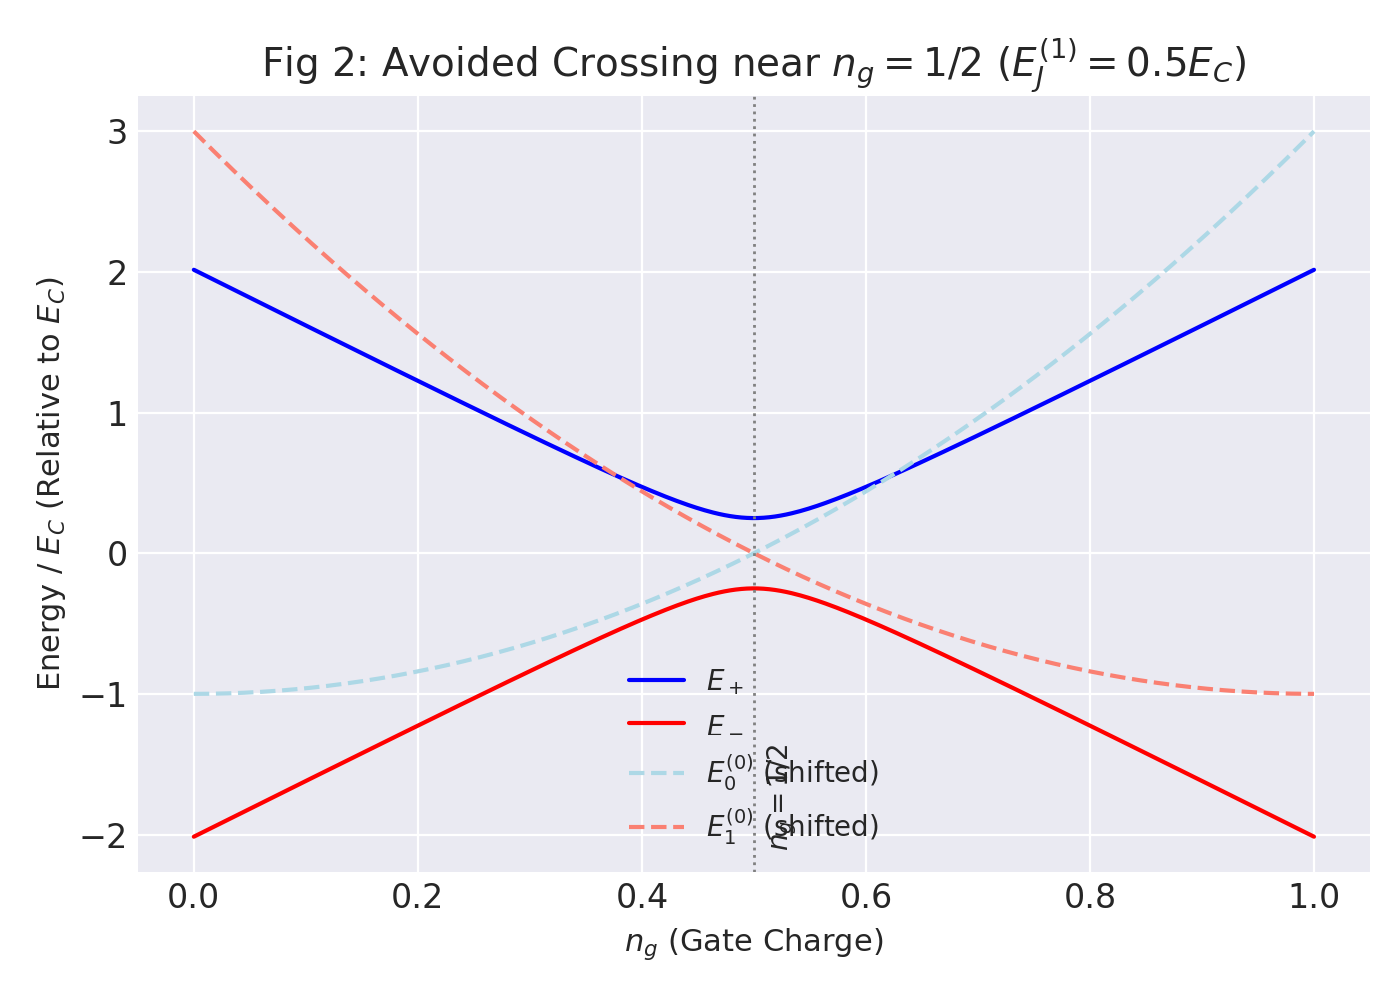
\includegraphics[width=0.8\textwidth]{fig_avoid_crossing.png}
    \caption[Avoided crossing near n\_g=1/2]{Energy levels near the \(n_g = 1/2\) degeneracy point. Dashed lines are the unperturbed energies \(E_0^{(0)}, E_1^{(0)}\). Solid lines show the actual energies \(E_{\pm}\) (Eq.~\ref{eq:charge_qubit_energies}), demonstrating the avoided crossing caused by the Josephson coupling \(E_J^{(1)}\).}
    \label{fig:avoided_crossing}
\end{figure}

What is the ground state \(|\psi_{GS}\rangle\) corresponding to \(E_{-}\)? It's a superposition \(|\psi_{GS}\rangle = c_0 |0\rangle + c_1 |1\rangle\). The probability of measuring charge \(N=0\) is \(P(N=0) = |c_0|^2\). Standard diagonalization of the \(2\times 2\) matrix gives:
\begin{equation}
P(N=0) = \frac{1}{2} \left( 1 + \frac{-\epsilon_0}{\sqrt{\epsilon_0^2 + (E_J^{(1)}/2)^2}} \right) = \frac{1}{2} \left( 1 - \frac{4 E_C (n_g - 1/2)}{\sqrt{[4 E_C (n_g - 1/2)]^2 + (E_J^{(1)}/2)^2}} \right)
\end{equation}
As we tune \(n_g\) across \(1/2\), this probability smoothly transitions from nearly 1 (mostly \(|0\rangle\) state for \(n_g \ll 1/2\)) to nearly 0 (mostly \(|1\rangle\) state for \(n_g \gg 1/2\)). At \(n_g = 1/2\), \(P(N=0) = 1/2\), an equal superposition. Figure~\ref{fig:charge_prob} shows this for a specific parameter choice.

\begin{figure}[h]
    \centering
    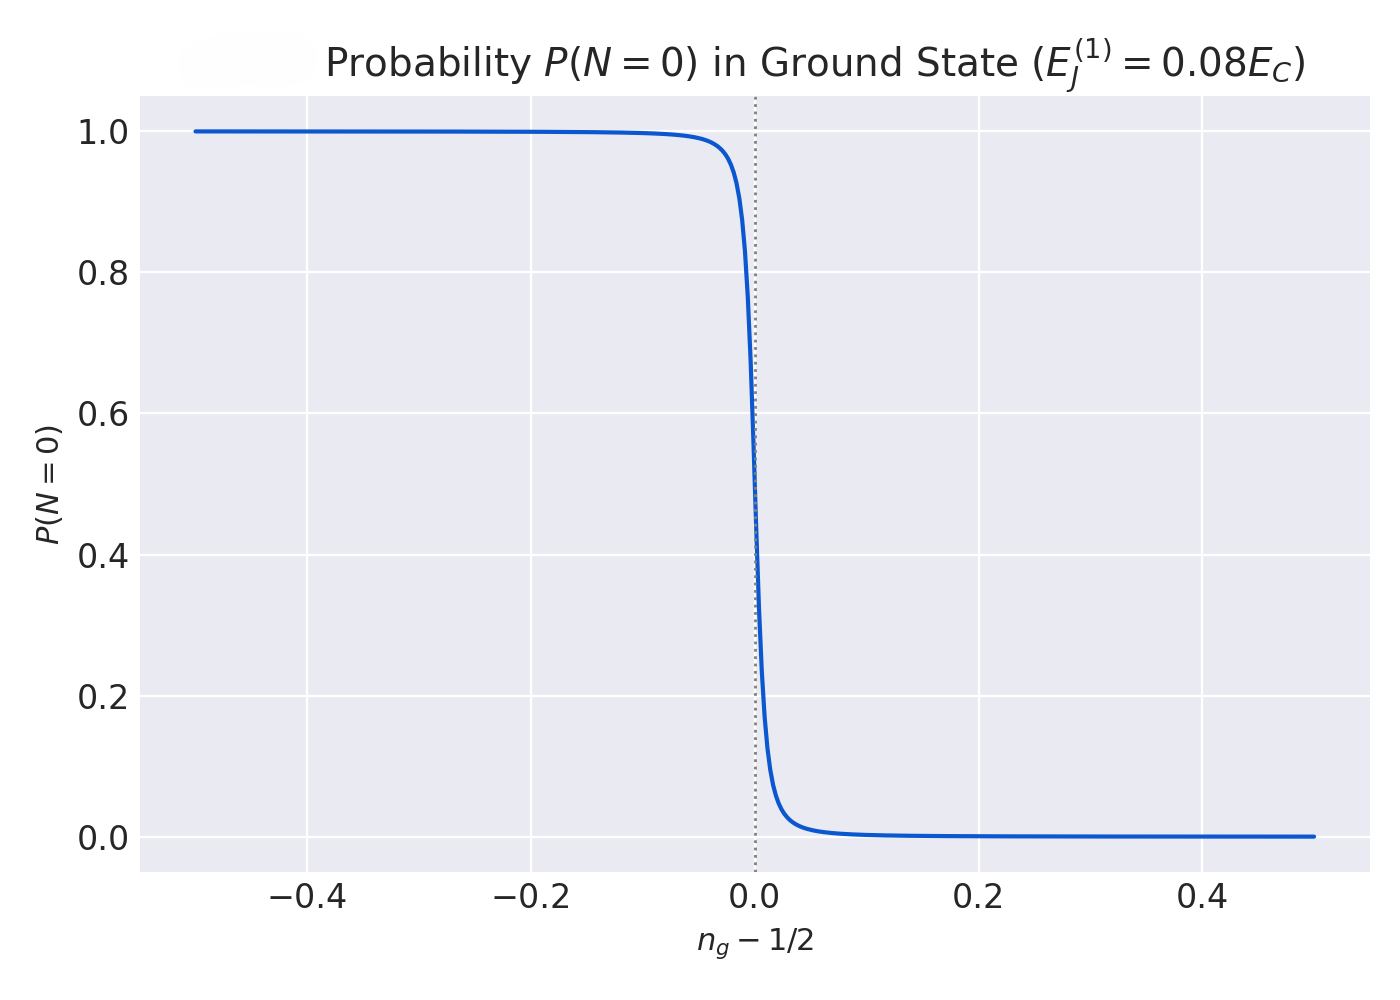
\includegraphics[width=0.8\textwidth]{fig_charge_prob.png}
    \caption[Ground state charge probability near n\_g=1/2]{Probability \(P(N=0)\) that the ground state has charge 0, plotted versus the deviation from the degeneracy point, \(x = n_g - 1/2\), for \(E_J^{(1)} = 0.08 E_C\). The sharp dependence on \(n_g\) highlights the qubit's sensitivity to gate charge fluctuations.}
    \label{fig:charge_prob}
\end{figure}

\begin{problem}[Problem \ref{chap:cpb}.a.iii, Part 2]
Calculate and plot the probability that the ground state has charge 0 as a function of \(n_g - 1/2\), for \(E_J^{(1)} = 0.08 E_C, E_J^{(2)} = 0\).
\end{problem}

This strong dependence on \(n_g\) is the Achilles' heel of the simple charge qubit – tiny fluctuations in \(n_g\) (charge noise) cause large fluctuations in the qubit's energy splitting, leading to rapid decoherence. This motivated the search for a less sensitive design.

\section[Case 2: Josephson Energy Dominates]{Case 2: Josephson Energy Dominates (\(E_J \gg E_C\))}
\label{sec:josephson_regime}

Now we flip the script: suppose the Josephson energies \(E_J^{(1)}, E_J^{(2)}\) are much larger than the charging energy \(E_C\). The system primarily wants to sit at the bottom of the potential well \(V(\phi) = -E_J^{(1)} \cos \phi - \frac{E_J^{(2)}}{2} \cos (2 \phi)\). The charging term \(4 E_C \hat{N}^2 = -4 E_C \frac{d^2}{d\phi^2}\) now acts like a small kinetic energy term, causing quantum fluctuations (zero-point motion) around the potential minimum. For simplicity, let's set the gate charge \(n_g = 0\). The Hamiltonian is:
\begin{equation}
\hat{H} = 4 E_C \hat{N}^2 - E_J^{(1)} \cos \hat{\phi} - \frac{E_J^{(2)}}{2} \cos (2 \hat{\phi})
\end{equation}

\subsection{Approximation near the Potential Minimum: The Harmonic Oscillator}
\label{subsec:ho_approx}

Assuming \(E_J^{(1)}, E_J^{(2)} > 0\), the potential \(V(\phi)\) has its primary minimum at \(\phi = 0\). For low-energy states, which will be localized near this minimum, we can approximate the potential using a Taylor expansion:
\[ V(\phi) = V(0) + V'(0)\phi + \frac{1}{2}V''(0)\phi^2 + \frac{1}{6}V'''(0)\phi^3 + \frac{1}{24}V^{(4)}(0)\phi^4 + \dots \]
At the minimum \(\phi=0\): \(V'(0)=0\), \(V'''(0)=0\). We have \(V(0) = -E_J^{(1)} - E_J^{(2)}/2\) and \(V''(0) = E_J^{(1)} + 2 E_J^{(2)}\). Keeping terms up to \(\phi^2\), the potential looks like a parabola:
\[ V(\phi) \approx V(0) + \frac{1}{2} (E_J^{(1)} + 2 E_J^{(2)}) \phi^2 \]
Plugging this into the Hamiltonian gives the harmonic oscillator Hamiltonian:
\begin{equation}
\hat{H}_{HO} \approx V(0) + 4 E_C \hat{N}^2 + \frac{1}{2} (E_J^{(1)} + 2 E_J^{(2)}) \hat{\phi}^2
\end{equation}
This is exactly the form \(\text{const} + \frac{\hat{p}^2}{2m^*} + \frac{1}{2} m^* \omega^2 \hat{x}^2\) if we identify \(\hat{p} \leftrightarrow \hat{N}\), \(\hat{x} \leftrightarrow \hat{\phi}\), effective mass \(m^* = 1/(8 E_C)\), and spring constant \(k = E_J^{(1)} + 2 E_J^{(2)}\). The characteristic frequency is \(\omega = \sqrt{k/m^*}\), which gives:
\begin{equation}
\omega = \sqrt{8 E_C (E_J^{(1)} + 2 E_J^{(2)})}
\label{eq:ho_freq}
\end{equation}
The energy levels, in this approximation, are those of a quantum harmonic oscillator:
\begin{equation}
E_n \approx E_n^{(HO)} = V(0) + \omega (n + 1/2), \quad n = 0, 1, 2, \dots
\label{eq:ho_energies}
\end{equation}
And the wavefunctions are the familiar Hermite-Gaussian functions:
\begin{equation}
\psi_n(\phi) \approx \psi_n^{(HO)}(\phi) = \left( \frac{\alpha^2}{\pi} \right)^{1/4} \frac{1}{\sqrt{2^n n!}} H_n(\alpha \phi) e^{-\alpha^2 \phi^2 / 2}
\label{eq:ho_wavefn}
\end{equation}


Specifically, the first three wavefunctions are:
\begin{align*}
\psi_0^{(HO)}(\phi) &= \left( \frac{\alpha^2}{\pi} \right)^{1/4} e^{-\alpha^2 \phi^2 / 2} \\
\psi_1^{(HO)}(\phi) &= \left( \frac{\alpha^2}{\pi} \right)^{1/4} \frac{1}{\sqrt{2}} (2\alpha\phi) e^{-\alpha^2 \phi^2 / 2} \\
\psi_2^{(HO)}(\phi) &= \left( \frac{\alpha^2}{\pi} \right)^{1/4} \frac{1}{\sqrt{8}} (4(\alpha\phi)^2 - 2) e^{-\alpha^2 \phi^2 / 2} 
\end{align*}
where $\alpha = \left( \frac{E_J^{(1)} + 2 E_J^{(2)}}{8 E_C} \right)^{1/4}$.


where \(H_n\) are the Hermite polynomials and \(\alpha\) determines the width of the ground state Gaussian.
% --- CORRECTED DEFINITION OF ALPHA ---
\begin{keyresult}[Harmonic Oscillator Parameter alpha]
The parameter \(\alpha\) characterizing the oscillator length scale is given by \(\alpha^2 = m^*\omega/\hbar\). With \(\hbar=1\), \(m^*=1/(8E_C)\) and \(\omega\) from Eq.~\ref{eq:ho_freq}, we get:
\[
\alpha^2 = \frac{\sqrt{E_J^{(1)} + 2 E_J^{(2)}}}{\sqrt{8 E_C}} \quad \implies \quad \alpha = \left( \frac{E_J^{(1)} + 2 E_J^{(2)}}{8 E_C} \right)^{1/4}
\]
\end{keyresult}
Note that a larger \(E_J/E_C\) ratio means a larger \(\alpha\), corresponding to a wavefunction more tightly localized near \(\phi=0\).

\begin{problem}[Problem \ref{chap:cpb}.b.i] 
Using the harmonic approximation, calculate the energy levels \(E_n\) and wavefunctions \(\psi_n(\phi)\) for the three lowest states (\(n=0, 1, 2\)).
\end{problem}

Let's visualize the probability densities \(p_n(\phi) = |\psi_n(\phi)|^2\). For the specific case \(E_C = (E_J^{(1)} + 2 E_J^{(2)}) / 800\), we find \(\alpha^2 = \sqrt{(E_J^{(1)} + 2 E_J^{(2)}) / (8 E_C)} = \sqrt{800/8} = \sqrt{100} = 10\). The densities for \(n=0, 1, 2\) will show the classic single, double, and triple peak structures (Figure~\ref{fig:ho_probs}).

\begin{figure}[h]
    \centering
    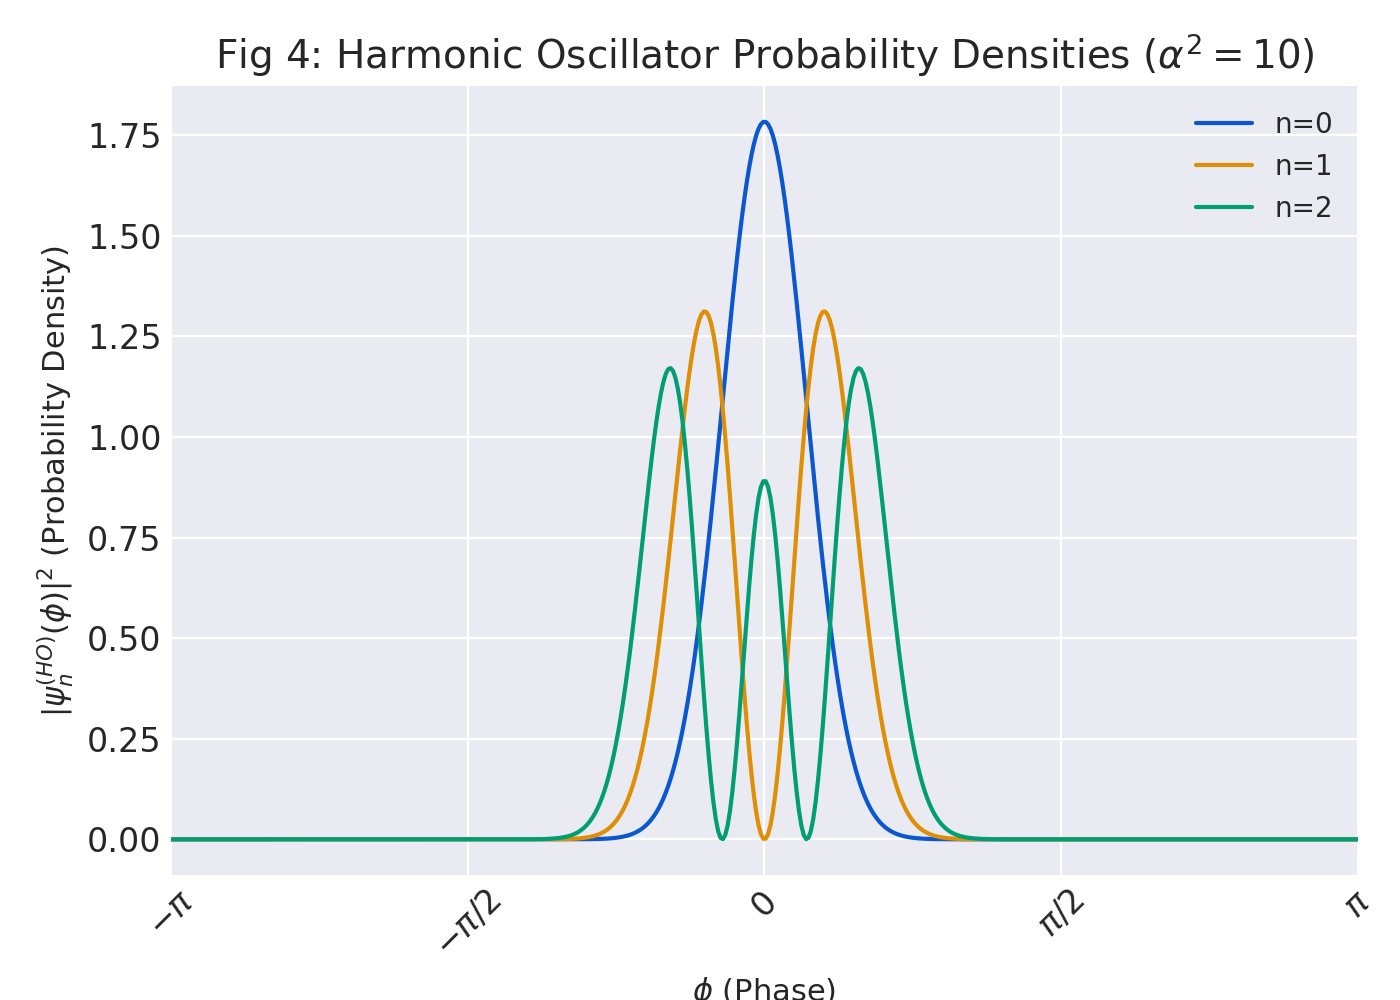
\includegraphics[width=0.8\textwidth]{fig_ho_prob.png}
    \caption[Harmonic oscillator probability densities]{Approximate probability densities \(p_n(\phi)=|\psi_n^{(HO)}(\phi)|^2\) for \(n=0, 1, 2\) using \(\alpha^2=10\). These states are localized near \(\phi=0\) and exhibit the characteristic node structure of harmonic oscillator eigenstates.}
    \label{fig:ho_probs}
\end{figure}

\begin{problem}[Problem \ref{chap:cpb}.b.ii] 
Calculate and plot \(p_n(\phi)\) for \(n=0, 1, 2\) using the parameter ratio \(E_C = (E_J^{(1)} + 2 E_J^{(2)}) / 800\).
\end{problem}

\subsection{Charge Uncertainty Revisited}
\label{subsec:charge_uncertainty}

If the phase \(\phi\) is now somewhat localized, the charge \(N\) must become uncertain. Let's quantify this for the ground state \(|n=0\rangle\). The average charge \(\langle \hat{N} \rangle_0 = \langle \psi_0 | (-i d/d\phi) | \psi_0 \rangle\) is zero, because \(\psi_0(\phi)\) is real and symmetric, so its derivative is antisymmetric, making the integral zero. The uncertainty is captured by the standard deviation \(\Delta N = \sqrt{\langle \hat{N}^2 \rangle_0 - \langle \hat{N} \rangle_0^2} = \sqrt{\langle \hat{N}^2 \rangle_0}\).

We can relate \(\langle \hat{N}^2 \rangle_0\) to the average kinetic energy in the ground state: \(\langle KE \rangle_0 = \langle \psi_0 | 4 E_C \hat{N}^2 | \psi_0 \rangle = 4 E_C \langle \hat{N}^2 \rangle_0\). For a harmonic oscillator, the average kinetic energy equals half the total energy (above the minimum), so \(\langle KE \rangle_0 = \frac{1}{2} (\hbar \omega / 2) = \omega/4\) (with \(\hbar=1\)). Therefore:
\[ \langle \hat{N}^2 \rangle_0 = \frac{\langle KE \rangle_0}{4 E_C} = \frac{\omega / 4}{4 E_C} = \frac{\omega}{16 E_C} \]
The charge standard deviation is \(\Delta N = \sqrt{\omega / (16 E_C)}\). Let's express this using the dimensionless parameter \(X = \sqrt{8 E_C / (E_J^{(1)} + 2 E_J^{(2)})}\), which is small in the transmon limit (\(E_J \gg E_C\)). Since \(\omega = \sqrt{8 E_C (E_J^{(1)} + 2 E_J^{(2)})} = \sqrt{8 E_C (8E_C/X^2)} = 8E_C/X\), we get:
\begin{equation}
\Delta N = \sqrt{\frac{(8 E_C / X)}{16 E_C}} = \sqrt{\frac{1}{2X}}
\end{equation}

\medskip
\noindent\textit{Caveat.}
The identity $\langle\mathrm{KE}\rangle=\langle\mathrm{PE}\rangle=\omega/4$
is exact only within the quadratic (harmonic) approximation to the cosine
potential.  Higher–order terms introduce corrections of order
$O[(E_C/E_J)^{3/2}]$—negligible in the deep-transmon regime
$E_J/E_C\!\gtrsim\!50$, but measurable once $E_J/E_C\lesssim10$.


As anticipated, when \(X\) is small (the transmon regime), \(\Delta N\) is large, signifying significant charge uncertainty (Figure~\ref{fig:delta_n}). This spread over many charge states is key to the transmon's insensitivity to charge noise.

\begin{figure}[h]
    \centering
    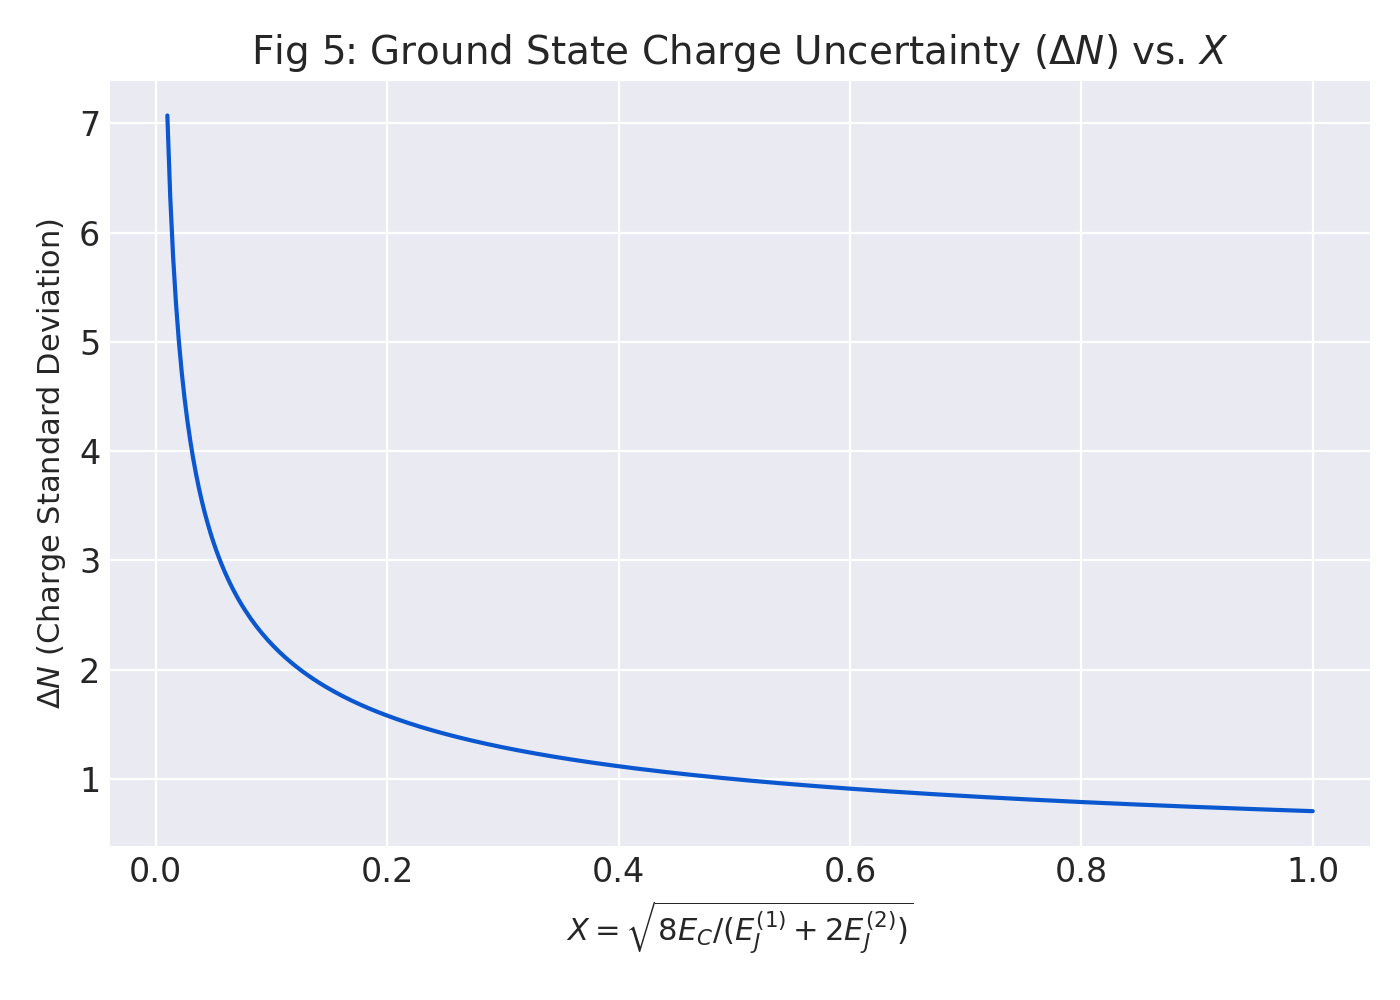
\includegraphics[width=0.8\textwidth]{fig_delta_n.png}
    \caption[Charge uncertainty vs. E\_C/E\_J ratio]{Charge standard deviation \(\Delta N = 1 / \sqrt{2 X}\) in the ground state, plotted against \(X = \sqrt{8 E_C / (E_J^{(1)} + 2 E_J^{(2)})}\). For small \(X\) (large \(E_J/E_C\), the transmon limit), \(\Delta N\) is large, indicating the state is a superposition of many charge eigenstates.}
    \label{fig:delta_n}
\end{figure}

\begin{problem}[Problem \ref{chap:cpb}.b.iii] 
Calculate the expectation value and variance (or standard deviation) of the charge \(\hat{N}\) in the ground state. Plot \(\Delta N\) as a function of \(X\).
\end{problem}

\subsection[Beyond the Parabola: Anharmonicity]{Beyond the Parabola: Anharmonicity}
\label{subsec:anharmonicity}

The harmonic oscillator approximation is useful, but the true potential \(V(\phi)\) is \textit{not} perfectly parabolic. The cosine terms have higher-order contributions, like \(\cos\phi \approx 1 - \phi^2/2 + \phi^4/24 - \dots\). The most important correction comes from the \(\phi^4\) term in the potential expansion:
\[ V_{pert} = \frac{1}{24} V^{(4)}(0) \hat{\phi}^4 = -\frac{E_J^{(1)} + 8 E_J^{(2)}}{24} \hat{\phi}^4 \]
We can treat this using first-order perturbation theory, calculating the energy shift \(\Delta E_n = \langle \psi_n^{(HO)} | V_{pert} | \psi_n^{(HO)} \rangle\). This requires the expectation value \(\langle n | \hat{\phi}^4 | n \rangle\). Using the properties of harmonic oscillator states (or ladder operators), one finds\footnote{The calculation yields \(\langle n | \hat{\phi}^4 | n \rangle = (\frac{\hbar}{2m^*\omega})^2 (6n^2+6n+3) = (\frac{4E_C}{\omega})^2 (6n^2+6n+3)\).}:
\[ \langle n | \hat{\phi}^4 | n \rangle = \left(\frac{4E_C}{\omega}\right)^2 (6n^2 + 6n + 3) \]
Plugging this in and simplifying using \(\omega^2 = 8 E_C (E_J^{(1)} + 2 E_J^{(2)})\), the first-order energy correction is:
\begin{equation}
E_n^{(1)} = -\frac{E_J^{(1)} + 8 E_J^{(2)}}{24} \left(\frac{16 E_C^2}{\omega^2}\right) (6n^2 + 6n + 3) = -C (6 n^2 + 6 n + 3)
\end{equation}
where the constant \(C\) is
\[ C = \frac{E_C (E_J^{(1)} + 8 E_J^{(2)})}{12 (E_J^{(1)} + 2 E_J^{(2)})} \]
Notice that the energy correction depends on \(n\) (specifically, quadratically). This means the energy levels are no longer equally spaced! The corrected energies are \(E_n \approx E_n^{(HO)} + E_n^{(1)}\).



The corrections for the first three levels are explicitly:
\begin{itemize}
    \item \(n=0\): \(E_0^{(1)} = -C (6(0)^2 + 6(0) + 3) = -3C\)
    \item \(n=1\): \(E_1^{(1)} = -C (6(1)^2 + 6(1) + 3) = -15C\)
    \item \(n=2\): \(E_2^{(1)} = -C (6(2)^2 + 6(2) + 3) = -C (24 + 12 + 3) = -39C\)
\end{itemize}
where $C = \frac{E_C (E_J^{(1)} + 8 E_J^{(2)})}{12 (E_J^{(1)} + 2 E_J^{(2)})}$.


\begin{problem}[Problem \ref{chap:cpb}.b.iv] 
Calculate the subleading correction to the first three energy levels (\(n=0, 1, 2\)).
\end{problem}

The difference in spacing between adjacent levels is called the \textit{anharmonicity}, typically defined as \(\alpha_{anh} = (E_2 - E_1) - (E_1 - E_0)\). Using our result for \(E_n^{(1)}\):
\begin{itemize}
    \item \(E_1^{(1)} - E_0^{(1)} = -C(6+6+3) - (-C(3)) = -15C + 3C = -12C\)
    \item \(E_2^{(1)} - E_1^{(1)} = -C(24+12+3) - (-C(15)) = -39C + 15C = -24C\)
\end{itemize}
So, the anharmonicity is \(\alpha_{anh} = (-24C) - (-12C) = -12C\).
\[ \alpha_{anh} = - E_C \frac{E_J^{(1)} + 8 E_J^{(2)}}{E_J^{(1)} + 2 E_J^{(2)}} \]
Since \(C > 0\), the anharmonicity is negative, meaning the energy spacing \textit{decreases} as you go up the ladder (\(E_2-E_1 < E_1-E_0\)). This is crucial: it allows us to use microwaves to target the \(0 \leftrightarrow 1\) transition (the qubit transition) without accidentally driving the \(1 \leftrightarrow 2\) transition, which would occur at a different frequency. Without anharmonicity, operating a qubit selectively would be impossible.

\begin{problem}[Problem \ref{chap:cpb}.b.v] 
Are the energy levels equidistant? Interpret your result.
\end{problem}

\section{An Exactly Solvable Case: Bridging the Regimes}
\label{sec:exact_solution}

It's rare in quantum mechanics to find exact solutions, but for a specific choice of parameters, this system obliges! Let \(n_g = 0\), \(E_J^{(1)} = E_J\), and choose the second Josephson term cleverly as \(E_J^{(2)} = E_J^2 / (4 E_C)\).
We emphasise that only the lowest eigenstate is closed-form; the excited manifold is still described by Mathieu functions and must be computed numerically.  Thus we reserve the phrase “exact solution’’ for the ground state alone.
The Hamiltonian becomes:
\[ \hat{H} = 4 E_C \hat{N}^2 - E_J \cos \hat{\phi} - \frac{E_J^2}{8 E_C} \cos (2 \hat{\phi}) \]
It turns out this Hamiltonian can be solved exactly, perhaps using techniques related to supersymmetric quantum mechanics or by finding a clever eigenstate ansatz. The result for the ground state is remarkably simple:

\begin{keyresult}[Exact Ground State for Special Parameters]
\label{res:exact_gs}
The exact ground state energy is:
\[ E_0 = -\frac{E_J^2}{8 E_C} \]
And the corresponding (unnormalized) wavefunction is:
\[ \psi_0(\phi) = A \exp\left( \frac{E_J}{4 E_C} \cos \phi \right) \]
where \(A\) is a normalization constant. This wavefunction is related to Mathieu functions.
\end{keyresult}
Notice that the ground state energy \(E_0\) matches the second-order perturbation result we found in the charge limit (Sec~\ref{subsec:charging_pert}) if we set \(E_J^{(1)}=E_J\) and \(E_J^{(2)}=0\) there. This suggests the formula might be more general than expected, but the wavefunction structure is specific to this parameter choice.



Let's compare this exact ground state energy $E_0 = -E_J^2 / (8 E_C)$ to the harmonic oscillator approximation from Section~\ref{subsec:ho_approx}. For the specific parameters $E_J^{(1)}=E_J$ and $E_J^{(2)} = E_J^2 / (4 E_C)$, the HO ground state energy (Eq.~\ref{eq:ho_energies} with $n=0$) is:
\begin{align*}
E_0^{(HO)} &\approx V(0) + \omega/2 \\
&= -(E_J^{(1)} + E_J^{(2)}/2) + \frac{1}{2}\sqrt{8 E_C (E_J^{(1)} + 2 E_J^{(2)})} \\
&= -(E_J + \frac{E_J^2}{8 E_C}) + \frac{1}{2}\sqrt{8 E_C (E_J + 2 \frac{E_J^2}{4 E_C})} \\
&= -(E_J + \frac{E_J^2}{8 E_C}) + \frac{1}{2}\sqrt{8 E_C E_J + 4 E_J^2} \\
&= -(E_J + \frac{E_J^2}{8 E_C}) + \sqrt{2 E_C E_J + E_J^2} 
\end{align*}
This approximate energy $E_0^{(HO)}$ clearly differs from the exact result $E_0$. In the limit of large $E_J/E_C$, the exact $E_0$ scales as $E_J^2$, while the $E_0^{(HO)}$ involves a term scaling as $\sqrt{E_J^2} \sim E_J$. In the opposite limit, small $E_J/E_C$, $E_0^{(HO)} \approx -E_J + \sqrt{2 E_C E_J}$, while the exact $E_0 \approx 0$. This highlights that while the HO approximation captures the physics well for $E_J \gg E_C$ (anharmonic oscillator), this specific potential allows for an exact solution that simplifies differently. The exact energy notably matches the second-order perturbation result $E_0^{(2)}$ from Section~\ref{subsec:charging_pert} if we set $E_J^{(1)}=E_J$ and $E_J^{(2)}=0$ in that formula, giving $E_0^{(2)} = -E_J^2 / (8 E_C)$.



\begin{problem}[Problem \ref{chap:cpb}.c] 
Find the exact ground state energy \(E_0\) and wavefunction \(\psi_0(\phi)\). Compare to results from parts (a) and (b). Plot the probability density \(p(\phi) = |\psi_0(\phi)|^2\) for \(E_J / E_C = 0.4, 4, 40\).
\end{problem}

To plot the probability density \(p(\phi) = |\psi_0(\phi)|^2\), we need to normalize the wavefunction. The normalization integral involves a standard function: \(\int_{-\pi}^{\pi} e^{z \cos\phi} d\phi = 2\pi I_0(z)\), where \(I_0\) is the modified Bessel function of the first kind. Here, \(z = E_J / (2E_C)\). So, the normalized probability density is:
\begin{equation}
p(\phi) = \frac{|\psi_0(\phi)|^2}{\int |\psi_0|^2 d\phi} = \frac{\exp\left( \frac{E_J}{2 E_C} \cos \phi \right)}{2 \pi I_0(E_J / (2 E_C))}
\end{equation}
Plotting this for different values of \(E_J / E_C\) (Figure~\ref{fig:exact_probs}) beautifully illustrates the transition:
\begin{itemize}
    \item For small \(E_J / E_C\) (like 0.4), the exponent is small, \(e^{\dots} \approx 1\), and \(p(\phi)\) is nearly uniform (charge-like behavior).
    \item For large \(E_J / E_C\) (like 40), the exponent is large, making the function sharply peaked around \(\phi=0\) where \(\cos\phi\) is maximum (transmon-like behavior).
\end{itemize}

\begin{figure}[h]
    \centering
    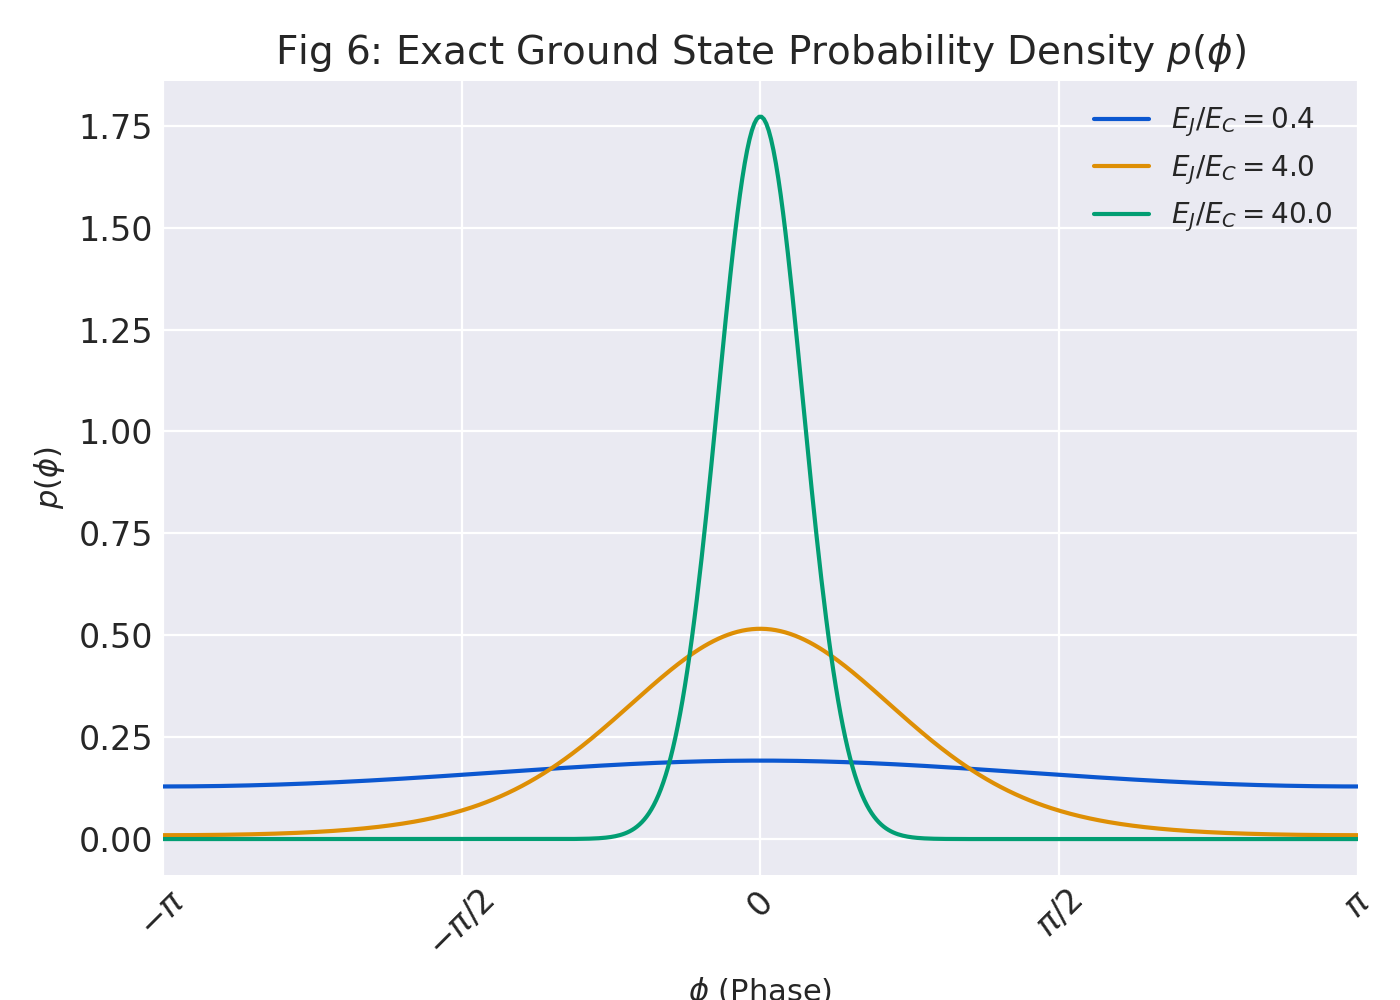
\includegraphics[width=0.8\textwidth]{fig_exact_prob.png}
    \caption[Exact ground state probability density]{Probability density \(p(\phi)\) for the exact ground state for \(E_J / E_C = 0.4\) (nearly flat), \(4\) (somewhat peaked), and \(40\) (sharply peaked). This clearly shows the evolution from a phase-delocalized state to a phase-localized state as the Josephson energy dominates.}
    \label{fig:exact_probs}
\end{figure}

\section{The Big Picture: Charge Qubits vs. Transmons}
\label{sec:interpretation}

Let's tie it all together. We've explored two main operational regimes of the Cooper Pair Box, governed by the crucial ratio \(E_J / E_C\) \cite{Kjaergaard2020}:

\begin{itemize}
    \item \textbf{The Charge Qubit Regime (\(E_C \gg E_J\))}:
        \begin{itemize}
            \item Physics dominated by charging energy. Eigenstates are close to definite charge states \(|N\rangle\).
            \item Operated near a charge degeneracy point (\(n_g \approx 1/2\)) using the two lowest states (\(|0\rangle, |1\rangle\)) mixed by \(E_J^{(1)}\).
            \item Key Feature: Avoided crossing in the energy spectrum (Fig~\ref{fig:avoided_crossing}).
            \item Major Drawback: The energy levels depend strongly on \(n_g\) (Eq~\ref{eq:charge_qubit_energies}). This makes the qubit extremely sensitive to environmental charge noise (fluctuating \(n_g\)), severely limiting its coherence time (how long it stays quantum).
        \end{itemize}

    \item \textbf{The Transmon Qubit Regime (\(E_J \gg E_C\))}:
        \begin{itemize}
            \item Physics dominated by Josephson energy. Eigenstates are localized in phase \(\phi\) near the potential minimum.
            \item Spectrum resembles a harmonic oscillator, but with a crucial \textit{anharmonicity} (\(\alpha_{anh} \approx -E_C\)) that makes level spacings non-uniform.
            \item Operated using the two lowest levels (\(n=0, 1\)) of this anharmonic oscillator.
            \item Key Advantage: Energy levels become almost independent of the gate charge \(n_g\). The \(n_g\) dependence is exponentially suppressed, scaling roughly as \(e^{-\sqrt{8 E_J / E_C}}\) \cite{Koch2007}. (See Figure~\ref{fig:transmon_levels}).
            \item Consequence: Greatly reduced sensitivity to charge noise, leading to much longer coherence times compared to the charge qubit. This robustness is why the transmon design became dominant in superconducting quantum computing.
        \end{itemize}
\end{itemize}
The anharmonicity (\(E_1-E_0 \neq E_2-E_1\)) in the transmon is essential – it allows us to precisely target the qubit transition with microwaves. The charge uncertainty (\(\Delta N \gg 1\)) is the *reason* for the charge noise insensitivity. The exact solution explored in Sec~\ref{sec:exact_solution} provides a snapshot of how the system smoothly interpolates between these two limiting behaviors as \(E_J/E_C\) is varied.

\begin{figure}[h]
    \centering
    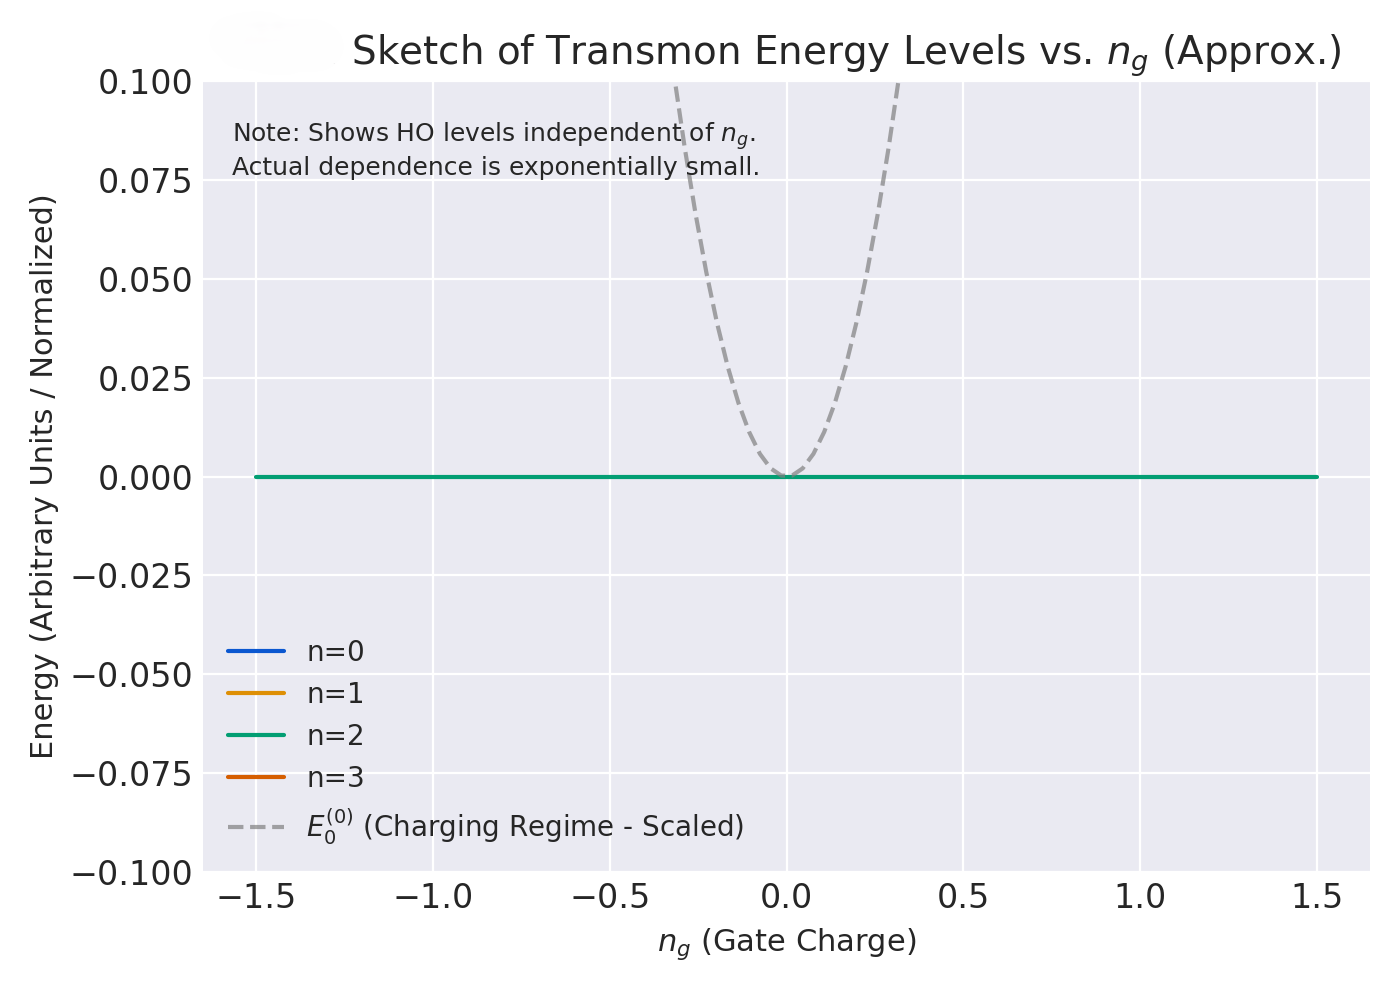
\includegraphics[width=0.8\textwidth]{fig_transmon_levels.png}
    \caption[Transmon energy levels vs. gate charge]{Sketch of typical transmon energy levels versus gate charge \(n_g\). Note how flat the levels are compared to the parabolic charge qubit levels (Fig~\ref{fig:charging_levels}). This flatness is the key to the transmon's improved coherence.}
    \label{fig:transmon_levels}
\end{figure}

\begin{problem}[Problem \ref{chap:cpb}.d] 
Interpret the results from parts (a)-(c). Include background on superconducting devices, define "charge qubit" and "transmon". Explain why anharmonicity is important for the transmon and why the transmon's reduced sensitivity to \(n_g\) fluctuations is advantageous. Use Ref~\cite{Kjaergaard2020} or similar.
\end{problem}


\section{Further Explorations}
\label{sec:further_problems}

For the curious reader, here are some avenues for further investigation:

\begin{enumerate}
    \item Verify the expression for \(\langle n | \hat{\phi}^4 | n \rangle\) used in the anharmonicity calculation. (Hint: Use ladder operators \(a, a^\dagger\)).
    \item What happens if \(n_g\) is not zero in the transmon regime? The term \(-8 E_C n_g \hat{N}\) appears in the Hamiltonian. Estimate its effect on the energy levels perturbatively.
    \item How does the potential \(V(\phi)\) change if \(E_J^{(1)}\) becomes negative? (This can happen in circuits with pi-junctions). Where is the minimum now?
    \item Research how the Josephson energy \(E_J\) can be tuned in practice, for example, by replacing the single junction with a SQUID loop threaded by magnetic flux.
    \item Carry out the normalization of the exact ground state wavefunction \(\psi_0(\phi)\) in Key Result~\ref{res:exact_gs}, confirming the role of the Bessel function \(I_0\).
\end{enumerate}

% --- Bibliography ---
% Using a simple bibliography environment
\begin{thebibliography}{9}
% Use consistent formatting for references
\bibitem{ReedSimonI} M. Reed and B. Simon, \textit{Methods of Modern Mathematical Physics, Vol. I: Functional Analysis}, Academic Press (1980). % Added subtitle for clarity
\bibitem{Kjaergaard2020} M. Kjaergaard, M. E. Schwartz, J. Braumüller, P. Krantz, J. I.-J. Wang, S. Gustavsson, and W. D. Oliver, "Superconducting Qubits: Current State of Play," \textit{Annual Review of Condensed Matter Physics} \textbf{11}, 369–395 (2020). % Added title, journal, volume, pages
\bibitem{Koch2007} J. Koch, T. M. Yu, J. Gambetta, A. A. Houck, D. I. Schuster, J. Majer, A. Blais, M. H. Devoret, S. M. Girvin, and R. J. Schoelkopf, "Charge-insensitive qubit design derived from the Cooper pair box," \textit{Physical Review A} \textbf{76}, 042319 (2007). % Added authors, title, journal, volume, pages
\end{thebibliography}

\end{document}
